% 数学发展史

参考\href{https://en.wikipedia.org/wiki/History_of_mathematics}{维基百科}.

\begin{figure}[ht]
\centering
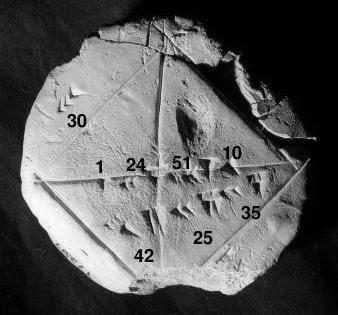
\includegraphics[width=6cm]{./figures/MathHi_1.png}
\caption{公元前 1800-1600 年的一块古巴比伦石碑上, 用 60 进制刻着 $\sqrt{2}$ 的值约为 $1 + 24/60 + 51/60^2 + 10/60^3 \approx 1.41421296\dots$, 误差约为 $-6.0\times10^{-7}$} \label{MathHi_fig1}
\end{figure}
